\documentclass[10pt]{article}
\usepackage[utf8]{inputenc}
\usepackage{graphicx}
\usepackage{float}
\usepackage{imakeidx}
\usepackage{amsmath}
\usepackage{hyperref}
\usepackage{graphicx}
\usepackage{float}
\usepackage{imakeidx}
\usepackage{amsmath}
\usepackage{url}
\usepackage[export]{adjustbox}
\usepackage{subcaption}
\title{CS414 Practical 2}
\author{Leandra Geldenhuys\\17534666\\\\Name here\\num here\\\\Name here\\num here}
\date{7 February 2017}

\usepackage{natbib}
\usepackage{graphicx}

\begin{document}

\begin{titlepage}
    \begin{center}
        \vspace*{1cm}
        
        \Huge
        \textbf{CS414 Practical 2\\Preliminary Design Review}
        
        \vspace{1.5cm}
        
        \Large
        Leandra Geldenhuys\\
        17534666\\
        \vspace{2.5cm}
        Daniel Robinson\\
        18361137\\
        \vspace{2.5cm}
        Leandra Geldenhuys\\
        17534666\\
        \vspace{4.5cm}
        %\vfill
        
        
        %\vspace{0.8cm}
        
        
        \Large
        Date: 7 February 2017
        
    \end{center}
\end{titlepage}


\tableofcontents
\listoffigures
\listoftables
\newpage
\section{Introduction}

\newpage

\section{Systems Overview}
In this section the mission objectives and requirements are specified.
\subsection{Mission Objectives}
In order to be deemed successful the CanSat system needs to complete the following missions:
\begin{itemize}
    \item The CanSat will be launched from approximately 1000m by a rocket.  The CanSat will then be ejected from the rocket.
    \item Measurements of air pressure and temperature will be taken during decent.
    \item These measurements will be transmitted at least once every second to the ground station.
    \item On the ground station the received data will be analysed.
\end{itemize}
\subsection{System Level Requirements}
The system has certain constraints and requirements it must adhere to:
\begin{itemize}
    \item The total mass should be between 490 and 510 grams.
    \item All components (except parachute, antenna and GPS) should fit inside a can with a height of 115 mm and 66 mm diameter.
    \item The container should fit inside a cylindrical envelope with a height of 310 mm and 66 mm diameter.
    \item System should use a passive control system, with a controlled decent speed between 8 and 11 m/s.
    \item All electronics should be enclosed, shielded from the environment and hard mounted.
    \item The system should be able to survive 15 Gs acceleration.
    \item The system should be powered by alkaline batteries which should be easily accessible.
    \item All materials used must be safe for personnel, equipment and the environment. 
\end{itemize}

\subsection{Architecture}

\newpage

\section{Sensor Subsystem Design}
In this section the sensors of the system is designed.
\subsection{Subsystem Requirements}
The sensors needs to adhere to certain requirements:
\begin{itemize}
    \item System needs to be able to read air pressure, temperature and determine its dynamic state.
    \item The system needs to wake up when CanSat is launched from the rocket.
    \item All sensors need to be able to withstand extreme weather conditions and up to 15Gs.
\end{itemize}
\subsection{CanSat Sensor System}
\subsubsection{Launch Recognition}
In order for the system to recognize when it has been launched from the rocket, a type of switch needs to be designed.   The switch will turn on the power system and enable the CanSat to start reading from the sensors and transmitting to the ground.
\subsubsection{Attitude and Dynamic State}
To measure the attitude of the CanSat, a three axes sensor is needed that provide attitude information, including roll, pitch and yaw.  The dynamic state can be determined using a gyroscope, accelerometer and magnetometer. 
\subsubsection{Air Pressure and Temperature}
The air pressure and temperature needs to be taken during the CanSat's decent.  
\subsection{Trade Studies and Selections}
\subsubsection{Launch Recognition}
Possible designs include contact switches, magnetic switches and optical sensors.  Keeping the extreme conditions the switch circuit will have to endure in mind, a strong, durable contact switch is the best option.  The switch chosen for this design is the B5112 Normally Closed Pushbutton Switch from Control Products Inc. (seen in Figure~\ref{fig:p}). These switches are covered with thermoplastic and can withstand temperatures between 10 and 105 degrees Celsius.  According the Control Products Inc, their switches perform well "under the wettest, and harshest environmental conditions" which makes it ideal for this application.  It measures 20.57x40.89x9.52mm.
\subsubsection{Attitude and Dynamic State}
There are various different models of gyroscopes, accelerometers and magnetometers available on the market,  For this application, size and weight is a huge factor in the selection process.  For this reason an 'all in one' solution was chosen.  The IvenSense MPU-9250 (seen in Figure~\ref{fig:att}) is a 9-axis MotionTracking device which consists of a gyroscope, accelerometer and magnetometer.  It can also connect to third-party sensors using $I^2C$ communication.  The sensor is very small, 3x3x1 mm and can withstand up to 10 000 Gs.
\subsubsection{Air Pressure and Temperature}
Again, there are many different models of pressure and temperature sensors available on the market.  It is important that the chosen sensor can be used for this application.  The Altimeter Module MS5607 (seen in Figure~\ref{fig:pres}) from Parallax reads pressure and temperature, is small (2.16x2.03mm) and is used for high altitude balloons and altitude hold for UAVs, which makes it ideal.  This sensor can also communicate with the IvenSense sensor via $I^2C$.

\begin{figure}[H]
\begin{subfigure}{0.5\textwidth}
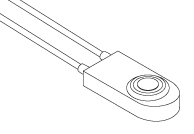
\includegraphics[scale =0.3]{3.png}
\caption{Pushbutton Switch.\\ Reproduced from \citep{cpi}.}
\label{fig:p}
\end{subfigure}
\begin{subfigure}{0.5\textwidth}
\centering
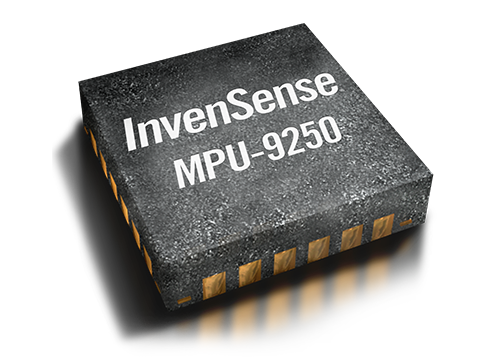
\includegraphics[scale =0.1]{2.png}
\caption{IvenSense MPU-9250. \\Reproduced from \citep{iven}.}
\label{fig:att}
\end{subfigure}
\begin{subfigure}{0.5\textwidth}
\centering
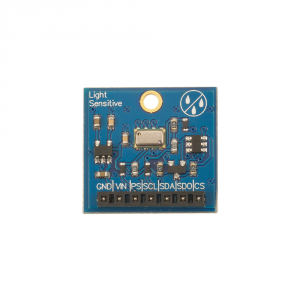
\includegraphics[scale =0.3]{1.png}
\caption{Altimeter Module MS5607. \\Reproduced from \citep{par}.}
\label{fig:pres}
\end{subfigure}
\caption{Sensors}
\end{figure}


\newpage

\section{Mechanical Subsystem Design}
\subsection{Overview}
\subsection{Key Trade Issues}
\subsection{Preliminary Mass Budget}

\newpage

\section{Communication and Data Handling Subsystem Design}
\subsection{Requirements}
\subsection{Processor and Memory Trade and Selection}
\subsection{Antenna Selection Criteria}

\newpage

\section{Electrical Power Subsystem Design}
\subsection{Components}
\subsection{Schematic}
\subsection{Power Source}

\newpage

\section{Flight Software Design}
\subsection{CanSat Flight Software Design}
\subsection{Flight Software Tasks}
\subsection{Software State Diagrams}

\newpage

\section{Ground Control System Design}
\subsection{Ground Station}
\subsection{Components and Connections}
\subsection{Requirements}

\newpage

\section{CanSat Integration and Test}
\subsection{Subsystem Level Testing Plans}
\subsection{Integrated Level Functional Testing Plans}
\subsection{Environmental Testing Plans}

\newpage

\section{Mission Operations}
\subsection{Preliminary Launch Day}
\subsection{Integrated Level Functional Testing Plans}
\subsection{Environmental Testing Plans}
\subsection{Possible Risks}
The risk matrix has been constructed.
\begin{figure}[H]
\centering
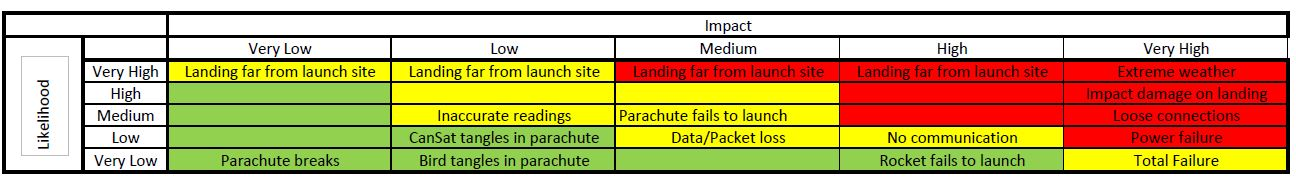
\includegraphics[scale =0.4]{risk.JPG}
\label{fig:risk}
\caption{Risk Matrix}
\end{figure}

\newpage

\section{Requirements Compliance}

\section{Conclusion}

\newpage
\bibliographystyle{plain}
\bibliography{references}

\end{document}
